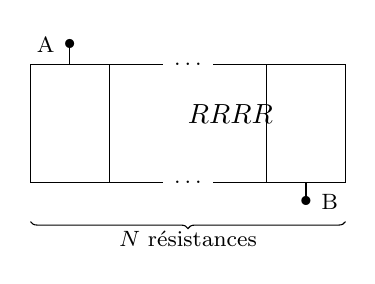
\begin{tikzpicture}[
	baseline=-1ex,
	scale=1,
	font=\footnotesize,
	]
	\draw (-1.5,.75)--++(0,.25)node{$\bullet$}node[left=2pt]{A};
	\draw (1.5,-.75)--++(0,-.25)node{$\bullet$}node[right=2pt]{B};
	\draw (-2,-.75)rectangle (-1,.75);
	\draw (2,-.75)rectangle (1,.75);
	\draw (-1,.75)--(1,.75)node[midway,fill=white,inner sep=4pt]{$\ldots$};
	\draw (-1,-.75)--(1,-.75)node[midway,fill=white,inner sep=4pt]{$\ldots$};
	\draw [decorate,decoration = {brace,mirror}] (-2,-1.25)--++(4,0)node[below,midway]{$N$ résistances};
	\resistanceV{shift={(-2,0)}}{$R$};
	\resistanceV{shift={(-1,0)}}{$R$};
	\resistanceV{shift={(1,0)}}{$R$};
	\resistanceV{shift={(2,0)}}{$R$};
\end{tikzpicture}